\documentclass[a4paper, 11pt, final, garamond]{book}
\usepackage{cours-preambule}

\raggedbottom

\makeatletter
\renewcommand{\@chapapp}{Travaux pratiques -- TP}
\makeatother

\let\SavedIndent\indent
\protected\def\indent{%
  \begingroup
    \parindent=\the\parindent
    \SavedIndent
  \endgroup
}
\setlength{\parindent}{0pt}

\begin{document}
\setcounter{chapter}{9}

\chapter{Suivi cin\'etique par spectrophotom\'etrie~: r\'eaction du cristal
violet avec la soude}

\section{Objectifs}

\begin{itemize}
    \item Revoir la technique de spectrophotométrie.
    \item Tracer un spectre d'absorption d'une solution colorée~: le cristal
        violet.
    \item Suivre la cinétique d'une réaction lente~: 
    \item Vérifier des conditions expérimentales de dégénérescence de l'ordre.
\end{itemize}

\section{S'approprier~: Rappels de spectrophotométrie}

Certaines espèces chimiques sont capables d'absorber la lumière UV ou visible.
Ainsi, est-il possible de relier l'intensité lumineuse transmise à une longueur
d'onde donnée à la concentration d'une espèce en solution par la \textbf{loi de
Beer-Lambert}~:
\begin{rprop}{Loi de \textsc{Beer-Lambert}}
    \[\boxed{A = \log\left(\frac{I_0}{I}\right) = \sum_{i=1}^{N}\epsilon_i \,
    \ell \, c_i}\]
    Avec~:
    \begin{itemize}
        \item $A$ est l'absorbance (adimensionnée). C'est une grandeur
            \textbf{additive}
        \item $I_0$ l'intensité lumineuse incidente (en $\si{W.m^{-2}}$)
        \item $I$ l'intensité lumineuse en sortie de cuve (en $\si{W.m^{-2}}$)
        \item $\epsilon_i$ le coefficient d'extinction molaire de l'espèce ${\rm
            X}_i$ à la longueur d'onde $\lambda$ (dépend de l'espèce chimique
            étudiée mais aussi marginalement du solvant et de la température)
        \item $\ell$ la largeur de la cuve traversée par le faisceau (en $\si{m}$)
        \item $c$ la concentration en l'espèce absorbante ${\rm X}_i$ (en
            $\si{mol.L^{-1}}$)
    \end{itemize}
\end{rprop}

Ici, on se limite à une unique espèce absorbante, tel que la relation de
Beer-Lambert devient
\[\boxed{A = \log\left(\frac{I_0}{I}\right) = \epsilon \, \ell \, c}\]

La valeur de $\epsilon \, \ell$ est bien souvent inconnue. Pour
obtenir $c_0$ connaissant $A_0$ de notre solution inconnue, il est donc
nécessaire de déterminer préalablement l'expression de la fonction $A=f(c)$.
Cette courbe est appelée \textbf{courbe d'étalonnage}. Elle est obtenue avec
l'ensemble des points de coordonnées $(A_i, c_i)$ obtenus à partir d'un ensemble
de solutions étalons $S_i$ de concentrations connues.

\section{Analyser}
\subsection{Préliminaires}

\begin{minipage}{0.7\linewidth}
    Les pictogrammes ci-contre sont présents sur le flacon contenant le cristal
    violet. Que signifient-ils~? Quelle précaution faut-il prendre~?
    Vous pourrez consulter \url{http://www.inrs.fr/media.html?refINRS=ED%204406}
\end{minipage}
\begin{minipage}{0.3\linewidth}
    \begin{center}
        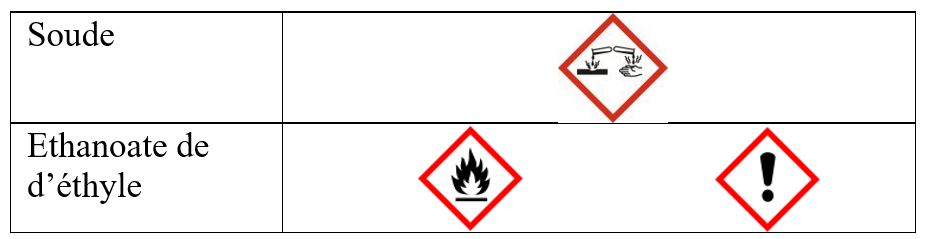
\includegraphics[width=\linewidth]{picto}
    \end{center}
\end{minipage}

\subsection{Etude cinétique de la réaction entre le cristal violet et la soude}

\subsubsection{Présentation}

On étudie maintenant la réaction entre le cristal violet (noté $\ce{CV^+}$,
c'est un ion complexe fortement coloré en violet dès que $\pH \geq 2$) et la
soude selon l'équation bilan~: 

\[\ce{CV^+_{(aq)} + OH^-_{(aq)} = CV-OH_{(aq)}}\]

Le produit $\ce{CV-OH}$ obtenu n'absorbe pas dans le visible alors que le
$\ce{CV^+}$ absorbe. On constatera donc une décoloration de la solution au cours
de la manipulation. On suppose que la réaction admet un ordre et que
l'\textbf{ordre global et les ordres partiels par rapport à chacun des réactifs
sont égaux à 0, 1 ou 2}.

\subsubsection{Données}

\begin{rdefi}{Données}
    \begin{itemize}
        \item Solution de cristal violet de concentration massique
            $c_{m}(\ce{CV}) = \SI{10,0}{mg.L^{-1}}$.
        \item Solution de soude de concentration molaire $c(\ce{OH}) =
            \SI{0,10}{mol.L^{-1}}$.
        \item Masse molaire du cristal violet~: $M(\ce{CV}) =
            \SI{408}{g.mol^{-1}}$.
    \end{itemize}
\end{rdefi}

\subsubsection{Étude des conditions expérimentales}

\begin{rexem}{Questions}
    \begin{enumerate}[label*=\protect\fbox{\arabic{enumi}}]
        \item Pourquoi peut-on penser qu'on peut suivre cette cinétique par
            spectrophotométrie~?
        \item Écrire la loi de vitesse de réaction. On appellera $v$ cette
            vitesse, $\alpha$ l'ordre partiel par rapport au cristal violet,
            $\beta$ celui par rapport à $\ce{OH^-}$ et $k$ la constante de
            vitesse de la réaction.
        \item En tenant compte des données, calculer les concentrations
            initiales respectives en cristal violet $c_0(\ce{CV})$ et en soude
            $c_0(\ce{OH})$ dans la cuve. Y a-t-il dégénérescence de l'ordre~?
            Modifier l'écriture de la loi de vitesse dans ce cas, en notant
            $k_{\rm app}$ la constante de vitesse apparente.
    \end{enumerate}
\end{rexem}

\subsubsection{Détermination de l'ordre partiel $\alpha$ par rapport au cristal
violet}

\begin{rexem}{Questions}
    Montrer que~:
    \begin{enumerate}[label*=\protect\fbox{\arabic{enumi}}, start=4]
        \item Si la réaction est d'ordre 1 par rapport au cristal violet, il
            faut tracer $\ln(A)=f(t)$ pour vérifier cette loi cinétique.
        \item Si la réaction est d'ordre 2 par rapport au cristal violet, il
            faut tracer $1/A=f(t)$ pour vérifier cette loi cinétique.
    \end{enumerate}
\end{rexem}

\subsubsection{Détermination de l'ordre partiel $\beta$ par rapport aux ions
hydroxydes}

On note $k_{\rm app}$ la constante de vitesse pour une concentration en ions
hydroxydes $[\ce{OH^-}]_{01}$ et $k_{\rm app}'$ la constante de vitesse pour une
concentration en ions hydroxydes $[\ce{OH^-}]_{02}=[\ce{OH^-}]_{01}/2$.

\begin{rexem}{Questions}
    \begin{enumerate}[label*=\protect\fbox{\arabic{enumi}}, start=6]
        \item Montrer qu'alors 
            \[\beta = \frac{\ln\left(\frac{k_{\rm app}}{k_{\rm app}'}\right)}{\ln(2)}\]
    \end{enumerate}
\end{rexem}

\section{Réaliser et valider}

\begin{NCror}[width=\linewidth]{Important}
    \begin{center}
        \bfseries
        Le port de la blouse fermée et des lunettes est obligatoire durant
        l'ensemble du TP. Les cheveux longs doivent être attachés.
    \end{center}
\end{NCror}

\subsection{Réalisation du spectre du cristal violet}

Nous allons dans un premier temps établir le spectre d'absorption du cristal violet. 

\begin{instruc}{Calibration du spectrophotomètre}
    \begin{itemize}
        \item Calibrer~; Appuyer sur \boxed{0/1} puis   *cuve vide~: valid. et *
            imprime~: escape.
        \item Quand le calibrage est terminé~: le spectro affiche~:
            «~absorbance~», etc
        \item Arrêter l'appareil~: \boxed{0/1}.
    \end{itemize}
\end{instruc}

\underline{Puis, redémarrer le spectro (sous contrôle du PC cette fois)}
\begin{itemize}
    \item Ouvrir Regressi
    \item Dans Fichier / nouveau choisir S250
    \item Choisir dans le menu du spectro le protocole de communication~:
        \textbf{S 250 I/PC}.
    \item Cliquer sur le bouton correspondant au spectro éteint. Le spectro se
        rallume alors (il faut quelques secondes~!).
\end{itemize}

\underline{Pour tracer des spectres~: utiliser spectre paramétrable
\SIrange{335}{900}{nm}}
\begin{itemize}
    \item Choisir des longueurs d'ondes variant de $400$ à $\SI{700}{nm}$ avec
        un pas de $\SI{6}{nm}$.
    \item Effectuer le zéro avec une cuve remplie d'eau distillée (dans le bon
        sens, face transparente dans le passage du faisceau lumineux et en
        évitant de poser ses doigts sur les faces par lesquelles le faisceau
        passe), en cliquant sur  BLANC. Le spectro trace une ligne (bleue) de
        zéro pour toutes les longueurs d'ondes.
\end{itemize}

Puis réaliser le spectre du cristal violet en remplissant la cuve au
$3/4$ de sa hauteur avec la solution, puis en cliquant sur SPECTRE.

\medskip

\begin{minipage}{0.7\linewidth} \underline{Pour exploiter le graphe}~:
    \begin{itemize}
        \item Basculer dans Regressi~: menu Sauver du logiciel du spectro et
            remplir ou non les renseignements demandés.
        \item Grâce au réticule, pointer la longueur d'onde de la valeur
            maximale. Imprimer la courbe après avoir retiré le zéro en $x$ et
            relié les points grâce à un lissage d'ordre 3 (dans le menu
            Coordonnées).
    \end{itemize}
    \begin{enumerate}[label*=\protect\fbox{\arabic{enumi}}, start=7]
        \item À quelle longueur d'onde doit-on travailler ensuite pour avoir un
            maximum de précision sur la mesure de l'absorbance~?
        \item Cette longueur d'onde vous semble-t-elle cohérente compte tenu de
            la coloration de la solution~? On rappelle le cercle chromatique
            ci-contre. 
    \end{enumerate}
\end{minipage}
\begin{minipage}{0.3\linewidth}
    \begin{center}
        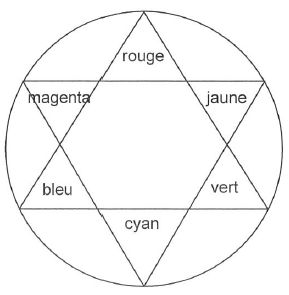
\includegraphics[width=\linewidth]{cercle}
    \end{center}
\end{minipage}

\subsection{Étude cinétique de la réaction entre le cristal violet et la soude}
\subsubsection{Détermination de l'ordre partiel $\alpha$ par rapport au cristal violet}

\textbf{a -- Protocole expérimental}~:

\begin{enumerate}
    \item Éteindre le spectro en débranchant la prise. Fermer Regressi
        complétement. 
    \item Allumer de nouveau le spectro en le rebranchant et en appuyant sur
        \boxed{0/1}. Aller jusqu'au bout de la procédure de calibration. 
    \item Eteindre le spectro en appuyant sur \boxed{0/1}. Le rallumer sous
        contrôle de l'ordinateur comme vu précédemment. Et choisir cette fois
        suivi cinétique. 
    \item Indiquer la valeur de $\lambda_{\max}$ pour déterminer la longueur
        d'onde à laquelle vous allez étudier l'évolution de l'intensité
        lumineuse.
    \item Faire le zéro avec une cuve remplie d'eau distillée en cliquant sur
        «~Z~». 
    \item Choisir ensuite 150 points, $Dt=\SI{4}{s}$, pour obtenir une durée
        d'expérience de 10 min environ. Valider. Puis refaire le blanc avec la
        cuve d'eau distillée en cliquant sur «~mettre le solvant avec la
        solution puis cliquer ici~».
\end{enumerate}
 
\begin{rrapp}{\includehand{-90}{.8cm}}
    \begin{center}
        \textbf{La suite de la manipulation doit être effectuée rapidement pour
            obtenir les premiers points, car dès le mélange entre le cristal
        violet et la soude, la cinétique démarre.}
    \end{center}
\end{rrapp}

Prélever à la finnpipette~: $\SI{1,8}{mL}$ de soude et $\SI{1,8}{mL}$ de Cristal
violet que vous déposerez successivement dans une cuve. Recouvrir de Parafilm
puis mélanger \textbf{rapidement}. Déposer cette dernière dans le spectro (dans
le bon sens~!) et lancer l'acquisition en cliquant sur «~mettre la cuve avec la
solution puis cliquer ici~».
 
\bigskip

\textbf{b -- Exploitation}~:

Une fois l'acquisition terminée, transférer les données sous Regressi en
cliquant sur l'icône prévue à cet effet. Créer les variables calculées
nécessaires, puis effectuer les régressions linéaires trouvées précédemment~;
les superposer avec deux échelles~: une échelle à gauche pour $lnA = \ln(A)$ et
une échelle à droite pour $invA = 1 / A$. Conclure sur l'ordre partiel par
rapport au cristal violet. Supprimer les zéros en ordonnées (menu coordonnées).

\medskip

Déterminer la constante apparente de vitesse de la réaction $k_{\rm app}$, ainsi
que le temps de demi-réaction $\tau_{1/2}$. Imprimer la courbe et les
modélisations effectuées. 

\subsubsection{Détermination de l'ordre partiel $\beta$ par rapport aux ions hydroxydes}

\begin{enumerate}
    \item Recommencer une nouvelle acquisition en prélevant~: $\SI{0,9}{mL}$ de
        soude, $\SI{0,9}{mL}$ d'eau distillée et $\SI{1,8}{mL}$ de Cristal
        violet. On a ainsi divisé par 2 la concentration de la soude et
        maintenue constante celle du cristal violet. 
    \item Vérifier l'ordre $\alpha$ que vous avez obtenu précédemment. 
    \item Déterminer expérimentalement la nouvelle constante apparente de
        vitesse de la réaction, notée $k_{\rm app}'$.
    \item En déduire l'ordre partiel $\beta$ par rapport à $\ce{HO^-}$~;
        l'arrondir à sa valeur entière la plus proche.
    \item Ne pas oublier d'imprimer les courbes obtenues, seuls repères pour
        l'examinataire. Vous prendrez soin de n'imprimer que les courbes et
        d'utiliser une impression noir et blanc.
\end{enumerate}

\section{Conclure}

\begin{enumerate}[label*=\protect\fbox{\arabic{enumi}}, start=9]
    \item Quels sont les ordres partiels expérimentaux~?
    \item Quel est l'ordre total de cette réaction~?
    \item Cette réaction suit-elle la loi de \textsc{Van't Hoff}~?
\end{enumerate}

\begin{NCror}[width=\linewidth]{Important}
    \begin{center}
        \bfseries
        En fin de séance, nettoyez votre paillasse, débranchez le
        spectrophotomètre et ne pas oublier d'enlever la cuve à l'intérieur du
        spectrophotomètre.
    \end{center}
\end{NCror}

% \begin{programme}{}
% 
% \vspace{1cm}
% \begin{itemize}
% \item Établir une loi de vitesse à  partir du suivi 
% temporel d'une grandeur physique. 
% \item Suivi cinétique de transformations chimiques 
% \item Suivi en continu d'une grandeur physique. 
% \item Mettre en Ïuvre une méthode de suivi temporel. 
% \item Exploiter les résultats d'un suivi temporel de 
% concentration pour déterminer les caractéristiques 
% cinétiques d'une réaction. 
% \item Proposer et mettre en Ïuvre des conditions 
% expérimentales permettant la simplification de la loi 
% de vitesse. 
% \item Pratiquer une démarche expérimentale pour 
% déterminer une concentration ou une quantité de 
% matière par spectrophotométrie UV-Visible.
% \end{itemize}
% \end{programme}

\end{document}
